\documentclass{article}
\iffalse
This file is protected by Copyright. Please refer to the COPYRIGHT file
distributed with this source distribution.

This file is part of OpenCPI <http://www.opencpi.org>

OpenCPI is free software: you can redistribute it and/or modify it under the
terms of the GNU Lesser General Public License as published by the Free Software
Foundation, either version 3 of the License, or (at your option) any later
version.

OpenCPI is distributed in the hope that it will be useful, but WITHOUT ANY
WARRANTY; without even the implied warranty of MERCHANTABILITY or FITNESS FOR A
PARTICULAR PURPOSE. See the GNU Lesser General Public License for more details.

You should have received a copy of the GNU Lesser General Public License along
with this program. If not, see <http://www.gnu.org/licenses/>.
\fi

\author{} % Force author to be blank
%----------------------------------------------------------------------------------------
% Paper size, orientation and margins
%----------------------------------------------------------------------------------------
\usepackage{geometry}
\geometry{
	letterpaper,			% paper type
	portrait,				% text direction
	left=.75in,				% left margin
	top=.75in,				% top margin
	right=.75in,			% right margin
	bottom=.75in			% bottom margin
 }
%----------------------------------------------------------------------------------------
% Header/Footer
%----------------------------------------------------------------------------------------
\usepackage{fancyhdr} \pagestyle{fancy} % required for fancy headers
\renewcommand{\headrulewidth}{0.5pt}
\renewcommand{\footrulewidth}{0.5pt}
\newcommand{\terminaloutput}[1]{\texttt{#1}}
\rhead{\small{ANGRYVIPER Team}}
%----------------------------------------------------------------------------------------
% Appendix packages
%----------------------------------------------------------------------------------------
\usepackage[toc,page]{appendix}
%----------------------------------------------------------------------------------------
% Defined Commands & Renamed Commands
%----------------------------------------------------------------------------------------
\renewcommand{\contentsname}{Table of Contents}
\renewcommand{\listfigurename}{List of Figures}
\renewcommand{\listtablename}{List of Tables}
\newcommand{\todo}[1]{\textcolor{red}{TODO: #1}\PackageWarning{TODO:}{#1}} % To do notes
\newcommand{\code}[1]{\texttt{#1}} % For inline code snippet or command line
%----------------------------------------------------------------------------------------
% Various packages
%----------------------------------------------------------------------------------------
\usepackage{hyperref} % for linking urls and lists
\usepackage{graphicx} % for including pictures by file
\usepackage{listings} % for coding language styles
\usepackage{rotating} % for sideways table
\usepackage{pifont}   % for sideways table
\usepackage{pdflscape} % for landscape view
%----------------------------------------------------------------------------------------
% Table packages
%----------------------------------------------------------------------------------------
\usepackage{longtable} % for long possibly multi-page tables
\usepackage{tabularx} % c=center,l=left,r=right,X=fill
\usepackage{float}
\floatstyle{plaintop}
\usepackage[tableposition=top]{caption}
\newcolumntype{P}[1]{>{\centering\arraybackslash}p{#1}}
\newcolumntype{M}[1]{>{\centering\arraybackslash}m{#1}}
%----------------------------------------------------------------------------------------
% Block Diagram / FSM Drawings
%----------------------------------------------------------------------------------------
\usepackage{tikz}
\usetikzlibrary{shapes,arrows,fit,positioning}
\usetikzlibrary{automata} % used for the fsm
\usetikzlibrary{calc} % For duplicating clients
\usepgfmodule{oo} % To define a client box
%----------------------------------------------------------------------------------------
% Colors Used
%----------------------------------------------------------------------------------------
\usepackage{colortbl}
\definecolor{blue}{rgb}{.7,.8,.9}
\definecolor{ceruleanblue}{rgb}{0.16, 0.32, 0.75}
\definecolor{drkgreen}{rgb}{0,0.6,0}
\definecolor{deepmagenta}{rgb}{0.8, 0.0, 0.8}
\definecolor{cyan}{rgb}{0.0,0.6,0.6}
\definecolor{maroon}{rgb}{0.5,0,0}
\usepackage{multirow}
%----------------------------------------------------------------------------------------
% Update the docTitle and docVersion per document
%----------------------------------------------------------------------------------------
\def\docTitle{Component Data Sheet}
\def\docVersion{1.5}
%----------------------------------------------------------------------------------------
\date{Version \docVersion} % Force date to be blank and override date with version
\title{\docTitle}
\lhead{\small{\docTitle}}

% find and replace: dev signal, devsignal -> \devsignal{}
\def\devsignal{devsignal}
% find and replace: Dev Signal, Dev signal, dev Signal, DevSignal -> \DevSignal{}
\def\DevSignal{DevSignal}


\def\comp{lime\_dac}
\edef\ecomp{lime_dac}
\def\Comp{Lime DAC}
\graphicspath{ {figures/} }

\begin{document}
\section*{Zipper Deprecation Notice:}
Beginning with OpenCPI Version 1.5, support for Lime Microsystems' Zipper card is now deprecated.
\section*{Summary - \Comp}
\begin{tabular}{|c|M{13.5cm}|}
	\hline
	\rowcolor{blue}
	                  &                  \\
	\hline
	Name              & \comp            \\
	\hline
	Worker Type       & Device           \\
	\hline
	Version           & v\docVersion \\
	\hline
	Release Date      & 4/2019 \\
	\hline
	Component Library & ocpi.assets.devices     \\
	\hline
	Workers           & \comp.hdl        \\
	\hline
	Tested Platforms  &
\begin{itemize}
  \item Epiq Solutions Matchstiq-Z1
  \item Digilent Zedboard/Zipper
  \item x86/Xilinx ML605/Zipper (FMC-LPC/FMC-HPC)
  \item x86/Altera ALST4/Zipper (HSMC A/B)
\end{itemize} \\
	\hline
\end{tabular}

\section*{Functionality}
\begin{flushleft}
	The Lime DAC device worker converts the OpenCPI WSI interface into the Lime LMS6002Dr2 Transceiver DAC interface. The data enters the worker in the control clock domain and is converted to the sample clock domain (DAC\_CLK).
\end{flushleft}

\section*{Worker Implementation Details}
\subsection*{\comp.hdl}
The clock domain crossing (CDC) from the OpenCPI control clock to the sample clock is performed using a two-clocked synchronizing FIFO. The WSI interface can be seen in Figure \ref{fig:ocpi_dac_interface}. The incoming 32 bit data contains one complex sample, with the lower 16 bits containing I and the upper 16 bits containing Q. Before it is loaded into the CDC FIFO, the 32 bit sample is reduced to 24 bits by taking the top 11 bits and rounding the 12th bit for both I and Q. The FIFO has a data width of 24 bits and depth of 64. Data is loaded into the FIFO when the upstream worker is ready and unloaded using TX\_IQ\_SEL. In the event that a sample cannot be unloaded from the FIFO, the \verb+underrun+ property is set and remains set until it is cleared. The FIFO output signals are then translated into the DAC interface.\par\bigskip
\begin{figure}[ht]
	\centering
	\includegraphics[scale=.5]{ocpi_dac_interface}
	\caption{WSI Interface: Control Clock Domain}
	\label{fig:ocpi_dac_interface}
\end{figure}
\noindent Figure \ref{fig:lime_dac_interface} shows the Lime DAC Interface in the sample clock domain. There are 14 output signals in the interface: DAC\_CLK(1), TX\_IQ\_SEL(1), and TXD(12). One data sample (I and Q) is clocked in every two DAC\_CLK cycles with TX\_IQ\_SEL serving as the qualifier for the I sample. The data width for the DAC is 12 bits and the data format is two's complement.\par\bigskip\bigskip
\begin{figure}[ht]
	\centering
	\includegraphics[scale=.6]{lime_dac_interface}
	\caption{Lime DAC Interface: Sample Clock Domain}
	\label{fig:lime_dac_interface}
\end{figure}
\noindent DAC\_CLK can originate from one of two sources based on the value of the parameters. The table below describes the valid settings.\par\bigskip
\noindent
\begin{scriptsize}
	\begin{tabular}{|M{5.3cm}|M{5.3cm}|M{5.3cm}|}
		\hline
		\rowcolor{blue}
		USE\_CLK\_IN\_p & USE\_CTL\_CLK\_p & DAC\_CLK    \\
		\hline
		True            & X                & TX\_CLK\_IN \\
		\hline
		False           & True             & ctl\_in.clk \\
		\hline
	\end{tabular}
\end{scriptsize}\par\bigskip
\noindent TX\_CLK can be driven by this worker by setting the DRIVE\_CLK\_p parameter or it can be driven from another source external to the worker.

\section*{Theory}
The main purpose of this worker is to perform a CDC for a data bus. The decision was made to implement the CDC using a two-clocked FIFO in an effort to target resources native the FPGA.

\section*{Block Diagrams}
\subsection*{Top level}
\begin{center}
	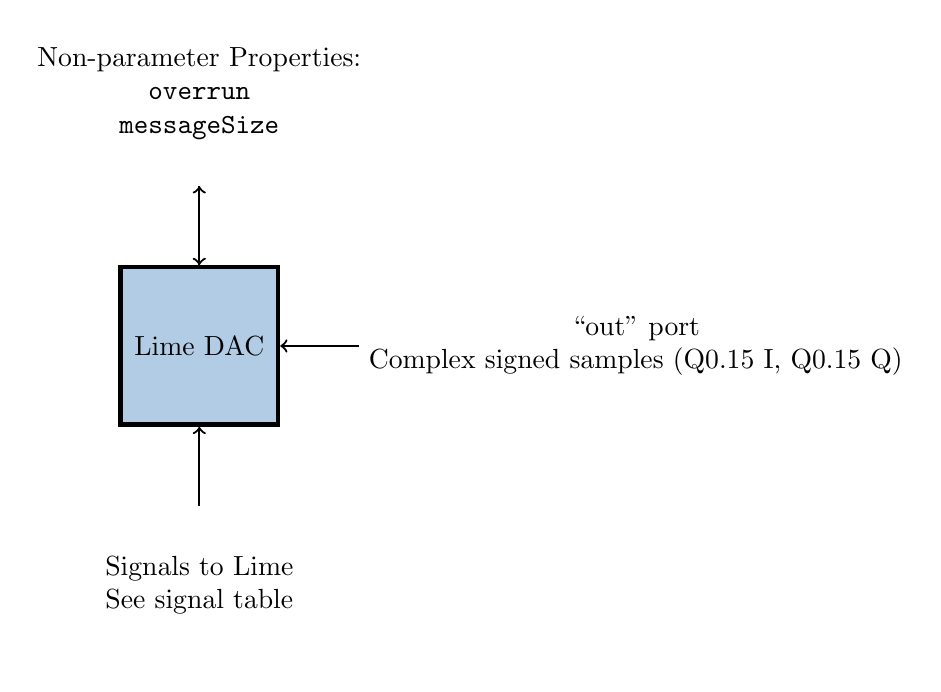
\begin{tikzpicture}[% List of styles applied to all, to override specify on a case-by-case
			every node/.style={
				align=center,  		% use this so that the "\\" for line break works
				minimum size=2cm	% creates space above and below text in rectangle
			},
			every edge/.style={draw,thick}
		]
		\node[rectangle,ultra thick,draw=black,fill=blue](R2){\Comp};
		\node[rectangle,draw=white,fill=white](R3)[below= of R2]{Signals to Lime \\ See signal table};
		\node[rectangle,draw=white,fill=white](R4)[right= of R2]{``out'' port \\ Complex signed samples (Q0.15 I, Q0.15 Q)};
		\node[rectangle,draw=white,fill=white](R5)[above= of R2]{Non-parameter Properties:\\\verb+overrun+\\ \verb+messageSize+\\};
		\path[->]
		(R3)edge []	node [] {} (R2)
		(R4)edge []	node [] {} (R2)
		(R2)edge []	node [] {} (R5)
		(R5)edge []	node [] {} (R2)
		;
	\end{tikzpicture}
\end{center}

\section*{Source Dependencies}
\subsection*{\comp.hdl}
\begin{itemize}
	\item assets/hdl/devices/lime\_dac.hdl/lime\_dac.vhd
	\item core/hdl/primitives/util/dac\_fifo.vhd
      \begin{itemize}
      	\item Performs the clock domain crossing between the control clock and sample clock domains
		\item assets/hdl/devices/lime\_adc.hdl/sync\_status.vhd
    		\begin{itemize}
			\item Generates the \textit{underrun} event when the DAC tries to unload a sample and the DAC FIFO is empty
		\end{itemize}
		\item core/hdl/primitives/bsv/imports/SyncFIFO.v
    		\begin{itemize}
		    	\item Two-clocked CDC FIFO
	    \end{itemize}
      \end{itemize}
\end{itemize}
\begin{landscape}

	\section*{Component Spec Properties}
	\begin{scriptsize}
		\begin{tabular}{|p{3.75cm}|p{1.25cm}|p{2cm}|p{2.75cm}|p{1.5cm}|p{1.5cm}|p{1cm}|p{6.62cm}|}
			\hline
			\rowcolor{blue}
			Name               & Type & SequenceLength & ArrayDimensions & Accessibility      & Valid Range & Default & Usage                                                                               \\
			\hline
			\verb+underrun+    & Bool & -              & -               & Volatile, Writable    & Standard    & -       & Flag set when DAC tries to send a sample and the DAC FIFO is empty. Once high, this flag is not cleared (i.e. set low) until the property is written to again (the flag clears regardless of write value, i.e. writing true or false both result in a value of false).\\
			\hline
		\end{tabular}
	\end{scriptsize}

	\section*{Worker Properties}
	\subsection*{\comp.hdl}
	\begin{scriptsize}
		\begin{tabular}{|p{2cm}|p{4cm}|p{1cm}|p{2cm}|p{2cm}|p{2cm}|p{2cm}|p{1cm}|p{3.95cm}|}
			\hline
			\rowcolor{blue}
			Type         & Name                 & Type & SequenceLength & ArrayDimensions & Accessibility & Valid Range & Default & Usage                                                                                                                  \\
			\hline
			Property     & \verb+fifo_depth+    & ULong& -              & -               & Parameter     & Standard           & 64      & Depth in number of samples of the control-to-DAC clock domain crossing FIFO. \\
			\hline
			Property     & \verb+IDATA_WIDTH_p+ & UShort&-              & -               & Parameter     & Standard           & 32      & \\
			\hline
			Property     & \verb+min_num_cp_clks_per_txen_events+ & UShort & - & -        & Initial, Readable & Standard       & 938     &
After every ZLM received on the \verb+event_in+ port, backpressure will be held on that port for one less than the number of control plane clock cycles specified by this property. This is done in order to ensure tx events are properly synchronized to the DAC clock without losing any events. Minimum required value is ceil(1.5 * control plane clock rate / DAC clock rate [use lowest expected DAC clock rate for your scenario]).
\\
			\hline
			Property     & \verb+other_present+ & Bool & -              & -               & Readable      & -           & -       & Not implemented. Flag to indicated presence of ADC worker                                                              \\
			\hline
			Property     & \verb+DRIVE_CLK_p+   & Bool & -              & -               & Parameter     & Standard    & 1       & Drive the clock sent to Lime (TX\_CLK). Some platforms do not connect TX\_CLK to the FPGA, making this parameter false \\
			\hline
			Property     & \verb+USE_CLK_IN_p+  & Bool & -              & -               & Parameter     & Standard    & 0       & Use copy of clock sent to Lime (TX\_CLK) as DAC\_CLK.                                                                  \\
			\hline
			Property     & \verb+USE_CTL_CLK_p+ & Bool & -              & -               & Parameter     & Standard    & 1       & Use control clock as DAC\_CLK. This is primarily for testing the component.                                            \\
			\hline
			Property     & \verb+divisor+       & -    & -              & -               & Writable      & -           & -       & Not implemented. Divider for DAC clock. This is primarily for testing the component.                                   \\
			\hline
			SpecProperty & \verb+underrun+      & -    & -              & -               & -             & -           & 0       & This property is set when the DAC tries to unload a sample and the DAC FIFO is empty.                                  \\
			\hline
		\end{tabular}
	\end{scriptsize}

	\section*{Component Ports}
	\begin{scriptsize}
		\begin{tabular}{|p{2cm}|p{1.5cm}|p{4cm}|p{1.5cm}|p{1.5cm}|p{10.75cm}|}
			\hline
			\rowcolor{blue}
			Name & Producer & Protocol           & Optional & Advanced & Usage                  \\
			\hline
			in   & False    & iqstream\_protocol & False     & -        & Complex signed samples (Q0.15 I, Q0.15 Q). \\
			\hline
			event\_in & False & tx\_event-prot   & False     & -        & TX on/off events. \\
			\hline
		\end{tabular}
	\end{scriptsize}

	\section*{Worker Interfaces}
	\subsection*{\comp.hdl}
	\begin{scriptsize}
		\begin{tabular}{|p{2cm}|p{1.5cm}|p{1.5cm}|p{1.5cm}|p{1.5cm}|p{13.23cm}|}
			\hline
			\rowcolor{blue}
			Type            & Name & DataWidth & Optional & Advanced & Usage                  \\
			\hline
			StreamInterface & in   & 32        & False    & -        & Complex signed samples (Q0.15 I, Q0.15 Q). This port ingests data and forces backpressure. Because both a ``pulling'' pressure from the DAC clock and potentially limited ``pushing pressure'' from this port exists, it is possible for a value to be clocked to the DAC while no new value was yet seen at the in port. This event is monitored via the \verb+underrun+ property.  \\
			\hline
			StreamInterface & event\_in  & -   & True     & -        & TX on/off events. \\
			\hline
			DevSignal & dev\_txen  & -   &      & -        &  txen-out-signals - Signal for controlling the Tx\_EN pin of the Lime transceiver device\\
			\hline
			DevSignal & dev\_tx\_event  & -   &      & -        &  lime-tx-event-signals - Bus interface signals to the lime\_spi.hdl worker, which subsequently controls the Tx\_EN register bit value.\\
			\hline
		\end{tabular}
	\end{scriptsize}\\ \\


	\section*{Signals}
	\scriptsize
	\begin{tabular}{|M{2.5cm}|M{1.5cm}|M{1.5cm}|M{14.5cm}|}
		\hline
		\rowcolor{blue}
		Name & Type & Width & Description \\
		\hline
		TX\_CLK & Output & 1 & Clock input to Lime \\
		\hline
		TX\_IQ\_SEL & Output & 1 & IQ Select to Lime \\
		\hline
		TXD & Output & 12 & Lime DAC data bus. IQ interleaved \\
		\hline
		TX\_CLK\_IN & Input & 1 & Copy of TX\_CLK sent to FPGA \\
		\hline
	\end{tabular}
\end{landscape}

		\section*{Control Timing and Signals}
		The Lime DAC device worker uses the clock from the Control Plane and Control Plane signals.\par\bigskip
		\noindent The latency through the worker from the input port to the DAC pins is 1 control clock cycle and 2 sample clock cycles. The data is loaded from the input port into the FIFO in one control clock cycle and unloaded to the DAC pins every other sample clock cycle (when TX\_IQ\_SEL is high).

\begin{landscape}
\section*{Worker Configuration Parameters}
\subsubsection*{\comp.hdl}
%\input{../../\ecomp.hdl/configurations.inc}
\section*{Performance and Resource Utilization}
\subsubsection*{\comp.hdl}
%\input{../../\ecomp.hdl/utilization.inc}
\end{landscape}
	\section*{Test and Verification}
	\begin{flushleft}
	 To be detailed in a future release.
	\end{flushleft}
	\section*{References}
	\begin{flushleft}
		\begin{itemize}
			\item[1)] LMS6002D Datasheet, www.limemicro.com
		\end{itemize}
	\end{flushleft}
\end{document}

